
\subsection{Link Failure Detection Using OpenFlow}
\label{subsec:pcnt}

% PCount Key Points: (1) measure packet loss inside the network, rather than E2E measurements.  (2) measure packet loss of link but can be more general. 
%    link failed if loss exceeds threshold, specified as a parameter.  threshold are packet loss at small time-scales (single w)


%\pcnt measures packet loss for a single link
%We consider a link as failed when the rate of packet loss exceeds a given threshold.  Because we focus on PMU applications that are sensitive to packet loss, our aim is to detect packet loss at 
%small timescales.  To this end, we present \pcnts, an algorithm that uses OpenFlow to detect link failures when and where
%they occur, inside the network.  In-network detection is used to reduce the time between when the loss occurs and when it is detected. In contrast, most previous work \cite{Almes99,Caceres99, 
%Friedl09} focuses on measuring end-to-end packet loss, resulting in slower detection times. 

%\pcnt estimates the rate of packet loss between an upstream node ($u$) and one or more downstream nodes.  
%For simplicity, our description of \pcnt assumes only a single adjacent downstream node, $d$. 
%For each window of length $w$, \pcnt estimates packet loss along $(u,d)$ by measuring the loss experienced by flows $M=\{f_1,f_2, ...,f_k\}$, specified as input, such that each $f_i \in M$
%traverses $(u,d)$, using the following steps: 

We present \pcnts, an algorithm that uses OpenFlow to detect link failures inside the network.  In-network detection is used to reduce the time between when packet loss occurs and when it is detected. 
Fast packet loss detection is crucial to the critical PMU applications that we target in this work, as they are particularly sensitive to packet loss. Most previous work \cite{Almes99,Caceres99, 
Friedl09} focuses on measuring end-to-end packet loss, resulting in slower detection times. 

\pcnt considers a link as failed when the rate of packet loss exceeds a threshold, given as input. For simplicity, our description of \pcnt assumes it measures packet loss over a single 
link, $(u,d)$.  At the end of the section we comment on how \pcnt easily generalizes to detect packet loss between multiple switches and non-adjacent switches.  

\pcnt estimates packet loss over a sampling window of length $w$.  For each $w$, \pcnt estimates packet loss along $(u,d)$ by measuring the aggregate loss rate 
experienced by flows $M=\{f_1,f_2, ...,f_k\}$ across link $(u,d)$, where $M$ is given as input, using the following steps: 
%specified as input, such that each $f_i \in M$ traverses $(u,d)$, using the following steps: 
\begin{enumerate}

	\item \textbf{Install rules (downstream) to count all tagged $f_i$ packets received at $d$.} \pcnt does so by installing a new flow table entry for each $f_i$ at $d$, 
	that matches packets using the identifier (i.e., the tag) applied at $u$ in step (2).  As noted in Section \ref{subsec:openflow}, for each flow table entry,
	OpenFlow automatically updates the packet counter each time a packet matches the flow table entry.
	
	
	\item \textbf{Tag (upstream) all packets from each $f_i \in M$.} Suppose $u$ uses flow table entry $e_i$ to match and forward flow $f_i$ packets. First, \pcnt generates
	a unique identifier (tag). Then, for each $f_i$, \pcnt creates a new flow table entry, $e_i'$, that is an exact copy of $e_i$ except that $e_i'$ embeds a the tag in the packet's 
	{\tt dl\_vlan} field. $e_i'$ is installed with a higher OpenFlow priority than $e_i$, ensuring that all flow $f_i$ packets are tagged.  


	\item \textbf{After $w$ time units, turn tagging off at $u$} by installing a copy of each $f_i$'s original flow table entry, $e_i$, but with a higher priority than $e_i'$.
	
	\item \textbf{Query $u$ and $d$ for packet counts} in order to compute the packet loss.  Each tagging rule is queried individually at $u$, while a single aggregate query (matching flows based
	on their the {\tt vlan\_id} field) is issued at $d$ to retrieve the packet counts of total packet count of all $f_i \in M$. 
	\footnote{We are unable to issue an aggregate query at $u$ because OpenFlow does not support query predicates specified over flow table entry actions.  In our case, it would be convenient if we could
	to specify an aggregate query of the form ``return statistics of all flow table entries that write identifier $x$ in the {\tt dl\_vlan} field''. }
	Before querying $d$, \pcnt waits time proportional to half the average RTT from $u$ to $d$, starting from the time step (3) completes, to ensure all in-transit packets are considered at $d$. 

	\item \textbf{Signal an alarm} if the estimated loss rate exceeds the input threshold.

	\item \textbf{Delete tagging and counting flow table entries} created in steps (1) and (2).
	
\end{enumerate}

Consider the example in Figure \ref{fig:intuition-example} and assume \pcnt monitors packet loss of both multicast flows traversing $(g,l)$; $f_b$ for primary tree $T_b$ (blue) 
and $f_c$ for primary tree $T_c$ (green). %-- traverse $(g,l)$ and we assume \pcnt measures packet loss of both flows. 
First, \pcnt selects a unique {\tt dl\_vlan} value (the identifier) and installs two flow table entries at $l$, one for $f_b$ and the other $f_c$. 
These flow table entries match packets based on the packet's multicast address and {\tt dl\_vlan} value.
Next, a flow table entry for $f_b$ and $f_c$ is installed upstream at $g$ that writes the {\tt dl\_vlan} identifier in each packet sent along the outgoing link to $l$.  After
$w$ seconds, tagging is turned off at $g$ and the flow statistics are read from $g$ and $l$.  Two individual flow statistic queries are sent to $g$, while a single aggregate query at $l$
gathers packet counts of the two flow table entries installed in the first step. %$l$ all flow table entries with a match field using the session's {\tt dl\_vlan} identifier.  
%gathers packet counts of all flow table entries with a match field using the session's {\tt dl\_vlan} identifier.  
Lastly, the packet counts are used to compute the loss rate and, if necessary, \pcnt raises an alarm if the measured loss rate during window $w$ exceeds the given threshold.  If not, a 
new \pcnt session is initiated, repeating the above steps.


%Tagging ensures that for each $f_i \in M$, \pcnt accounts for all packets dropped between $u$ and $d$ during $w$. %That is, \pcnt measures packet loss
%Tagging ensures that for monitored flow \pcnt accounts for all packets dropped during $w$. %That is, \pcnt measures packet loss
%Returning to our earlier generic example where \pcnt monitors link $(u,d)$
Tagging ensures that for monitored flow \pcnt accounts for all packets dropped during $w$. %That is, \pcnt measures packet loss
However, in some cases \pcnt may be configured to monitor a subset of flows traversing a monitored link because doing so can reduce the time required to compute packet loss, since 
$k+1$ statistic queries are required when monitoring $k$ flows.  For example, in Figure \ref{fig:intuition-example} \pcnt may only monitor $f_b$'s packet loss along $(g,l)$.  As a result,
only a single read statistics request needs to be sent to $g$ rather than two statistic queries if $f_c$ were also monitored.  However, monitoring a subset of flows means that
\pcnt does not account for packet loss of unmonitored flows.  In Section \ref{subsec:eval-pcount} we use simulations to explore how adjusting the number of monitored flows 
affects the  speed and accuracy of packet loss estimates.


%Doing so can boost packet loss detection time and reduce switch flow table size, at the cost of reducing \pcnt accuracy (from $100\%$ when all flows are monitored).
%Faster detection time are the result of processing fewer statistic queries at $u$ in Step 4 ($k'$ rather than $k$ queries), while scarce flow table space
%(Section \ref{subsec:openflow}) is made available since $k'$, rather than $k$, tagging and counting flow table entries are installed at $u$ and $d$, respectively.
%results from fewer having sending fewer statistic queries Detection time improves $u$ must process one statistics query per monitored flow; reduce forwarding table size at $u$ and $d$ since, for each monitored flow, a copy of the corresponding flow table entry is made at $u$ and $d$,
%In Section \ref{subsec:eval-pcount} we use simulations to explore how \pcnt accuracy can be traded for faster processing time. % by modifying the number of flows \pcnt monitors.

Although \pcnt sends instructions simultaneously to start tagging each $M$ flow (step 2) and, likewise, sends all $k$ messages in parallel to stop tagging (step 3), in practice
these actions are unlikely to be executed at the same time. %\pcnt cannot guarantee that these actions are issued at the exact same time (in fact this is quite unlikely). 
The implication is that across each $f_i \in M$ the start and stop time of $w$ is not perfectly synchronous.  This does not affect the accuracy of \pcnt packet loss measurements,
provided that all tagged packets that will eventually reach the downstream node do so before that node is queried.
%because our tags ensure that for each $f_i \in M$ both $u$ and $d$ consider exactly the same set of packets, excluding, of course, packets that are dropped at $u$ or dropped along
%the path from $u$ to $d$.  In fact, tags ensure that for each $f_i \in M$, \pcnt accounts for all packets dropped between $u$ and $d$ during the time $u$ tags packets.

%{\it need to copy each $e_i$ because may have different actions (outports) at $u$ or $d$}:

%We can issue an aggregate query at $u$ based on the priority but this would rely on no other flows having the same priority.

{\bf \pcnt Extensions.} 
%No changes are required for \pcnt to monitor packet loss between non-adjacent switches nor to measure packet loss between more than two switches. In this first case, consider
No changes are required for \pcnt to monitor packet loss between non-adjacent switches. Consider the case where \pcnt 
measures packet loss between two non-adjacent switches $a$ and $b$.  The \pcnt actions at $a$ and $b$ are the same as described above, while the forwarding at any switches along
a path between $a$ to $b$ disregards (as they already do) any tag applied at $a$ or $b$.  In this scenario, \pcnt measures packet loss of a path rather than that of a single link.

\pcnt can also be used to monitor packet loss between multiple (possibly) non-adjacent switches. Consider the example topology in Figure \ref{fig:pcount-multipoint}, where \pcnt measures
packet loss between $u$ and downstream nodes $d_1$ and $d_2$. For simplicity, we assume a single flow multicasts packets from $u$ to $d_1$ and $d_2$. \pcnt installs 
a rule to tag packets at $u$, leaves $v$ is unchanged, and installs a rule at $d_1$ and $d_2$ to count packets tagged at $u$. Then, \pcnt (as its only modification) queries $u$, $d_1$, and $d_2$
for their packet counts.

Notice that by comparing packet counts between $u$, $d_1$, and $d_2$, packet loss of links $(u,v)$, $(v,d_1)$, and $(v,d_2)$ can all be estimated using network tomography techniques \cite{Bu02}.
For example, if $u$ and $d_1$ have the same
packet counts but $d_2$ counts fewer packets than $u$, we can infer packet loss incurs along $(v,d_2)$.  This approach provides the same coverage (scope of packet loss measurements) as an alternative
approach that creates three separate \pcnt sessions between $(u,v)$, $(v,d_1)$, and $(v,d_2)$, but does do so using fewer measurement points. 
%Using fewer measurement points, this provides the same scope of packet loss measurements if separate \pcnt sessions were created between $(u,v)$, $(v,d_1)$, and $(v,d_2)$.  
We later find in our simulations (Section \ref{subsec:eval-pcount}) that monitoring a large number of flows
using a single link incurs high processing time at network switches, suggesting that the savings projected here of running a single \pcnt session between multiple switches can provide 
significant savings. 

\begin{figure}
  \centering
   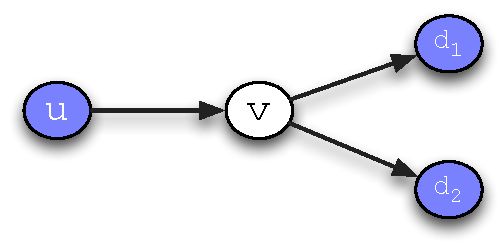
\includegraphics[scale=0.75]{figs/multicast/pcount-multipoint.pdf}
\caption{Example topology used to explain how \pcnt can be used to monitor packet loss between multiple non-adjacent switches.}
\label{fig:pcount-multipoint}
\end{figure}



%{\it 2/6/14 include: (a) write as if only monitoring a link and then, at the end of section, comment on how it can be extend to monitor multiple measurement points, (b) how threshold determined?}
